%
% File acl2021.tex
%
%% Based on the style files for EMNLP 2020, which were
%% Based on the style files for ACL 2020, which were
%% Based on the style files for ACL 2018, NAACL 2018/19, which were
%% Based on the style files for ACL-2015, with some improvements
%%  taken from the NAACL-2016 style
%% Based on the style files for ACL-2014, which were, in turn,
%% based on ACL-2013, ACL-2012, ACL-2011, ACL-2010, ACL-IJCNLP-2009,
%% EACL-2009, IJCNLP-2008...
%% Based on the style files for EACL 2006 by 
%%e.agirre@ehu.es or Sergi.Balari@uab.es
%% and that of ACL 08 by Joakim Nivre and Noah Smith

\documentclass[11pt,a4paper]{article}
\usepackage[hyperref]{acl2021}
\usepackage{times}
\usepackage{latexsym}
\usepackage{titlesec}
\usepackage{amsmath}
\usepackage{color,soul}
\setcounter{secnumdepth}{5}
\renewcommand{\UrlFont}{\ttfamily\small}
\usepackage{graphicx}
\graphicspath{{./images/}}
\usepackage[parfill]{parskip}

% This is not strictly necessary, and may be commented out,
% but it will improve the layout of the manuscript,
% and will typically save some space.
\usepackage{microtype}

\aclfinalcopy % Uncomment this line for the final submission
%\def\aclpaperid{***} %  Enter the acl Paper ID here

%\setlength\titlebox{5cm}
% You can expand the titlebox if you need extra space
% to show all the authors. Please do not make the titlebox
% smaller than 5cm (the original size); we will check this
% in the camera-ready version and ask you to change it back.

\newcommand\BibTeX{B\textsc{ib}\TeX}

\makeatletter
\renewcommand\paragraph{%
    \@startsection{paragraph}{4}{0mm}%
        {-\baselineskip}%
        {.5\baselineskip}%
        {\normalfont\normalsize\bfseries}}
\makeatother

\title{BigGreen at SemEval-2021 Task 1: \\
Lexical Complexity Prediction with Assembly Models}

\author{
  Aadil Islam\\
  Department of Computer Science\\
  Dartmouth College\\
  \texttt{aadil.islam.21@dartmouth.edu}
}

\date{}

\begin{document}
\maketitle
\begin{abstract}
  Here, I will write the abstract. This will be even briefer than the small description that I've previously submitted.
\end{abstract}

\section{Introduction}

\begin{itemize}
  \item Why lexical complexity prediction is important in the real world, namely via applications to readability, text simplication, etc.
  \item What the previous 2016 and 2018 SemEval tasks aimed to accomplish, the assumptions of said tasks, compared to this year's task, namely transition from binary task and probabilistic component to use of 5-point Likert scale. Do not go into findings from 2016 and 2018 tasks, yet.
  \item What models we submitted, overview of the sections of this paper, and a link to GitHub repo of our code.
\end{itemize}

\section{Related Work}

\begin{itemize}
  \item What previous papers showed (Mc Laughlin 1969, Dale and Chall 1948, Shardlow 2013, Paetzold and Specia 2016, Yimam et al. 2018).
  \item What 2016 task showed, overall findings of the authors, and shortcomings. 
  \item What 2018 task showed, overall findings of the authors, and shortcomings.
  \item What specific approaches from the above inspired us, namely our feature set, our use of BERT, and our ensembling techniques. Basically, substantiating our choices.
\end{itemize}

\section{Datasets}

\subsection{CompLex Dataset}

\begin{itemize}
  \item What advantages of CompLex Dataset are over past datasets.
  \item Number of instances breakdown (table) of single token (train, trial, test) and multi token (train, trial, test) by subcorpus (bible, biomed, europarl).
  \item Complexity distribution breakdown (table) of single token (train, trial, test) and multi token (train, trial, test) by subcorpus (bible, biomed, europarl).
  \item Mention that whenever we perform cross-validation upon each train set, we always stratify by class and corpus.
  \item Show actual samples that inspired us to pick particular features. 
  \begin{itemize}
    \item Eg. showing easy vs. difficult target words with respect to term frequency.
    \item Eg. showing easy vs. difficult target words with respect to it being proper noun or not.
    \item Eg. showing easy vs. difficult target words with respect to context (show the complexities of a target word under different contexts)
    \item ...
  \end{itemize}
\end{itemize}

\subsection{External Datasets}

\begin{itemize}
  \item Briefly credit external corpora used to extract term frequency-based features:
  \item English Gigaword corpus, Google Books Ngram Dataset (version 2) via PhraseFinder API \citep{phrasefinder}, British National Corpus (BNC), SUBTLEXus.
\end{itemize}

\section{BigGreen Systems \& Approaches}

In this section, we overview information fed to the feature engineering-based system, and the training strategies for the feature learning-based model. We also describe techniques for ensembling their predictions for each subtask. Note that the fitted models for the single word subtask are then harnessed for the multi-word expression subtask.

\subsection{Feature Engineering-based System}

\subsubsection{Feature Extraction}

The feature extraction procedure aims to capture a breadth of information pertaining to the target word and its context. The majority of features appear to follow heavily right-skewed distributions, perhaps due to governance of Zipf's law over the multitude of word frequency-based features we consider. This prompts us to consider both the logged and unlogged versions of each feature. For the multi-word expression subtask, features are extracted independently for the head and tail words, with they and their \textit{sums} being included in the feature set.

\paragraph{Lexical Features}

These are features based on lexical information about the target word:

\begin{itemize}
  \item \textbf{Word length}: the length of the target word.
  \item \textbf{Number of syllables}: the number of syllables in the target word, computed using the Syllables library\footnote{\url{https://github.com/prosegrinder/python-syllables}}.
  \item \textbf{Is acronym}: whether the target word is a sequence of capital letters.
\end{itemize}
  
\paragraph{Semantic Features}

These are features describing the meaning of the target word:

\begin{itemize}
  \item \textbf{WordNet features}: the number of hyponyms and hypernyms in WordNet \citep{Fellbaum:2005}.
  \item \textbf{GloVe word embeddings}: we extract 300-dimension embeddings pre-trained on Wikipedia-2014 and Gigaword \citep{pennington2014glove} for each (lowercased) target word. 
  \item \textbf{GloVe context embeddings}: we obtain the average 300-dimension GloVe word embedding over each token in the given sentence.
  \item \textbf{ELMo word embeddings}: we extract 1024-dimension embeddings pre-trained on the 1-Billion-Word-Benchmark corpus \citep{Peters:2018} for each target word. Observe that these are \textit{contextualized} embeddings, unlike the GloVe embeddings.
  \item \textbf{InferSent context embeddings}: we obtain 4096-dimension InferSent embeddings \citep{conneau-EtAl:2017:EMNLP2017} for each sentence.
\end{itemize}

\paragraph{Phonetic Features}

These features compute the likelihood that consecutive soundable segments comprising a target word would show up in the English language. Before extraction, we empirically estimate the ground truth transition probabilities between any two units (phonemes or characters) in the English language using the Gigaword corpus. 

\begin{itemize}
  \item \textbf{Phoneme transition probability}: we consider the minimum, maximum, average, and standard deviation over the set of estimated transition probabilities of the target word's phoneme bigrams.
  \item \textbf{Character transition probability}: analogous to the extraction procedure for phoneme transition probability, but over \textit{character} bigrams.
\end{itemize}

\paragraph{Word Frequency and N-gram}

These features are expressly included due to their expected  importance as predictors, as indicated by general takeaways from CWI 2016 (Malmasi and Zampieri, 2016). 

\textbf{Gigaword}: This serves as the primary corpus from which we extract word frequency measurements pertaining to the target word. These include term frequency (with and without lemmatizing the target word), the sum of the frequencies of each byte pair encoding (BPE), and the summed frequencies of bi-grams and tri-grams containing the target word. These features are complemented with their corresponding IDF-based analogues, and out-of-vocab (OOV) words in the sentence are counted.

\textbf{Google Books Ngram Dataset}, \textbf{British National Corpus}, \& \textbf{SUBTLEXus}: These corpora are used to extract secondary word frequency, bi-gram, and tri-gram measurements.

\paragraph{Syntactic Features}

These are features that assess the syntactic structure of the sentence in relation to the target word. Certain features rely on the construction of a constituency parse tree for the target word's context, which we obtain using a Stanford CoreNLP pipeline \citep{manning-EtAl:2014:P14-5}.

\begin{itemize}
  \item \textbf{Part of speech (POS)}: the part of speech tag predicted using NLTK's generic $\text{pos\_tag}$ function \citep{Loper02nltk:the}.
  \item \textbf{Depth of parse tree}: this measures the maximum depth of the parse tree.
  \item \textbf{Depth of target word}: this measures the distance between the target word and the parse tree's root node.
  \item \textbf{Is proper}: whether the target word is a proper noun/adjective, which we detect using capitalization of the first character.
\end{itemize}

\paragraph{Readability Metrics}

These comprise a variety of readability tests that are applied on the target word's context, capturing low-level traits such as total word count, total syllable count, etc. Interestingly, certain readability tests count the \textit{difficult} words in a given sentence by assuming rules as to what makes a given word complex—the Dale-Chall readability formula \citep{10.2307/1473669} checks a given word against a predetermined list of familiar words. This inspires us to conduct multiple readabililty tests via the Textstat library\footnote{\url{https://github.com/shivam5992/textstat}}, including Flesch-Kincaid grade level, Gunning Fog index, and SMOG index.

\subsubsection{Feature Selection}

For the single word subtask, we try selecting features using a combination of filter and wrapper methods. Our intention is to also leverage any successful techniques in the multi-word expression subtask, where we must select head-specific and tail-specific features.

\paragraph{Filter Methods}

\textbf{Variance}: Features are initially screened by the variance of their distribution, with those lower than a threshold of 0.01 being deemed constant or quasi-constant, and removed. 

\textbf{Mutual Information}: Features are ranked by their mutual dependence with lexical complexity, and the top-$k$ features are selected. We tune $k$ by evaluating linear regression models fitted on the top-$k$ features, settling on $k=300$. See Figure \ref{fig:mi}.

\begin{figure}
  \centering
  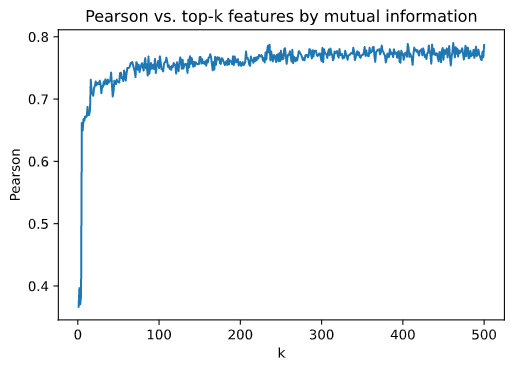
\includegraphics[scale=0.4]{mi.png}
  \caption{\label{fig:mi} Performances of LR fitted on top-k features by mutual information (with 5-fold cross-validation).}
\end{figure}

\textbf{Variance Inflation Factor (VIF)}: VIF is computed for each feature to measure contributed multicollinearity. Note that we omit this particular filter method for the submitted model, for the sake of optimizing Pearson correlation.

\paragraph{Wrapper Methods}

\textbf{Forward Feature Selection (FFS)}: Beginning with an empty feature set, each subsequent iteration appends a new feature to the existing feature set that offers the best Pearson correlation. We end the algorithm when the last added feature fails to sufficiently improve Pearson correlation.

\paragraph{Embedded Methods}

\textbf{Lasso \& Elastic Nets}: We consider these linear models during the subsequent training phase, which use L1 and L1/L2 regularization, respectively, to shrink regression coefficients of lesser important features \textit{during} fitting. Lasso \citep{Tibshirani.x} is intruiging due to its ability to reduce the high dimensionality of our feature set (relative to training set size) during fitting. Elastic Net \citep{10.2307/3647580} may succeed particularly in the presence of highly intercorrelated features.

\subsubsection{Training}

Prior to training, we standardize all features to have approximately zero mean and unit variance. For the single word subtask, we fit Linear Regression, Lasso Regression, Elastic Net Regression, Support Vector Regression (with linear kernel),  Support Vector Regression (with radial basis function kernel), K-Nearest Neighbors Regression, and XGBoost Regression models. 

After identifying the best performing model in terms of Pearson correlation, we mitigate the imbalanced nature of the target variable, ie. the multitude of class-1,2,3 samples and relative lack of class-4,5 samples. We devise a sister version of our top-performing model, fit upon a \textit{reduced} training set containing fewer class-1,2,3 samples. We tune the exact percentages removed from each class by performing cross-validation on the training set.

\subsection{System based on Feature Learning and Transfer Learning}

Based on our prior observations for samples possessing the same target word but different contexts, we hypothesize that lexical complexity draws on the target word's relationship to its context. Our existing handcrafted feature set relies heavily upon target word-specific features, resulting in a cursory analysis of context encapsulating the target word. Beyond existing N-gram and syntactic features, we seek an alternative approach for feature learning using deep learning approaches.

\subsubsection{Architecture}

LSTM-based approaches have been used successfully to model the contexts of target words in previous works \citep{hartmanndossantos2018nilc}. However, an issue with a standalone LSTM is that it is capable of reading tokens of an input sentence sequentially in a single direction. This inspires us to use an Transformer-based approach \citep{DBLP:journals/corr/VaswaniSPUJGKP17}, model architecures capable of processing sentences as a whole (instead of word-by-word) by applying \textit{attention} mechanisms over input sentences. Attention weights are useful as they can be interpreted as a measurement of learned relationships between words in a given sentence. BERT \citep{DBLP:journals/corr/abs-1810-04805} is one such language representation model that can be used for a variety of natual language understanding (NLU) tasks.

Multi-Task Deep Neural Network (MT-DNN) proposed by \citet{liuetal2019multitask} offers state-of-the-art results for a variety of NLU tasks by incorporating the benefits of both multi-task learning and language model-pretraining. MT-DNN initializes its shared text encoding layers using a pre-trained BERT model, whose later layers we intend to fine-tune for the lexical complexity subtasks.

We initialize MT-DNN with the BERT base model (cased), and fine-tune the model for 5 epochs, leaving any hyperparameters to their defaults.

\subsubsection{Input Layer}

Data is fed to the model's input layer in \textit{PremiseAndOneHypothesis} format, where the premise and hypothesis are sentence and target word (or expression for the multi-word expression subtask), respectively. The data is then tokenized by a BERT Tokenizer, backed by the HuggingFace tokenizers library \citep{wolf_etal_2020_transformers}.

\subsubsection{Output Layer}

The fine-tuned model's output layer returns the predicted lexical complexity for a given target word/expression. In addition, we aim to examine the behaviors of BERT's 144 attention heads, as interpretation of attention maps may provide insight into relevant linguistic features learned by the model, as \citep{DBLP:journals/corr/abs-1906-04341} demonstate.

\subsection{Ensembling}

To combine the 2 sets of predictions obtained from our best performing feature engineering-based regression model (from fitting on the \textit{full} and \textit{reduced} training sets, respectively), we default to using the \textit{full} predictions. We then tune a threshold, where predictions higher than the threshold (ie. likely of class-4,5 samples) being overwritten with their \textit{reduced} predictions. Lastly, we compute a weighted average ensemble of these predictions with those of our MT-DNN model to obtain a final set of predictions for the single word subtask. 

For the multi-word expression subtask, we harness the fitted feature engineering and feature learning-based models from the single word subtask by predicting the lexical complexities for the head and tail words each. We then compute a weighted average ensemble of these predicted complexities \textit{and} the predictions of the MT-DNN model trained on multi-word expressions.

\section{Results}

\begin{table*}[t]
  \centering
  \begin{tabular}{lcccc}
  \hline \textbf{Model} & \textbf{Pearson} & \textbf{Rank} & \textbf{Spearman} & \textbf{MAE} \\ \hline
  Linear Regression	& 0.7347 & - &	0.6993 &	0.0669 \\
  Forward Feature Selection (FFS)	& 0.7313 & - &	0.7053 & 0.0671 \\
  Lasso (alpha=0.0001) &	0.7352 & - &	0.7042 & 	0.0667 \\
  ElasticNet (alpha=0.001) &	0.7396 & - &	0.7122 &	0.0662 \\
  SVM (kernel=linear, C=0.001) &	0.7254 & - &	0.6970 &	0.0678 \\
  SVM (kernel=rbf, C=1, gamma=0.001) &	0.7392 & - &	0.7066 &	0.0668 \\
  KNN (k=20, weights=distance) &	0.7156 & -	& 0.6914 &	0.0710 \\
  \hline
  XGBoost (\textit{full}) &	0.7589 & - &	0.7220 &	0.0645 \\
  XGBoost (\textit{reduced}) &	0.7456 & - &	0.7157 &	0.0751 \\
  XGBoost (\textit{full}+\textit{reduced}) & 0.7576 & - & 0.7220 & 0.0646 \\
  MT-DNN & 0.7484 & -	& 0.7044 & 0.0664 \\
  Ensemble (submission) & 0.7749 & 8 of 54 & 0.7294 & 0.0629 \\
  \hline
  Best competition results & 0.7886 & & 0.7425 & 0.0609 \\ 
  \hline
  \end{tabular}
  \caption{\label{tab:single-word-results} Test set results for single word subtask. }
\end{table*}

\begin{table*}[t]
  \centering
  \begin{tabular}{lcccc}
  \hline \textbf{Model} & \textbf{Pearson} & \textbf{Rank} & \textbf{Spearman} & \textbf{MAE} \\ \hline
  Head predicted complexity & 0.7164 & - & 0.7305 & 0.1281 \\
  Tail predicted complexity & 0.7188 & - & 0.7416 & 0.1306 \\
  MT-DNN & 0.7890 & - & 0.7649 & 0.0766 \\
  Ensemble (post-competition) & 0.8290 & *14 of 37 & 0.8120 & 0.0857 \\
  Ensemble (submission) & 0.7898 & 25 of 37 & 0.7769 & 0.0903 \\
  \hline
  Best competition results & 0.8612 & &  0.8548 & 0.0616 \\ 
  \hline
  \end{tabular}
  \caption{\label{tab:multi-word-results} Test set results for multi-word expression subtask. (* projection)}
\end{table*}

Here, we present the performances of BigGreen's systems on test sets for the single and multi-word expression subtasks. See Tables \ref{tab:single-word-results} and \ref{tab:multi-word-results}.

\section{Analysis}

\subsection{Performance}

For feature selection, we find success in selecting the top-300 features by mutual information \textit{and} removing constant/quasi-constant features. The pruned feature set is then passed to both our wrapper/embedded methods and a variety of regressors for model comparison, where we find an XGBoost regressor \citep{DBLP:journals/corr/ChenG16} (with hyperparameters tuned using grid search) to excel consistently for the single word subtask.

We ensemble the predictions of our two sister XGBoost regressors and MT-DNN model accordingly, yielding a final set of predictions for the single word subtask. Performances are reported in Table \ref{tab:single-word-results}, where we rank in the top 15\% by Pearson. For the multi-word expression subtask, performances are reported in Table \ref{tab:multi-word-results}. Note that for this subtask our submitted predictions differ from our post-competition predictions. We \textit{previously} used a training procedure resembling that for the single word subtask: (1) filter methods for feature selection, (2) XGBoost for regression, and (3) ensembling with MT-DNN. We hypothesize that the fewer number of training samples available for multi-word expression subtask contributed to the previous procedure's lackluster performance. This inspired us to incorporate the predictive capabilities of our fitted single word subtask models, yielding superior post-competition results.

\subsection{Feature Contribution}

\begin{figure}
  \centering
  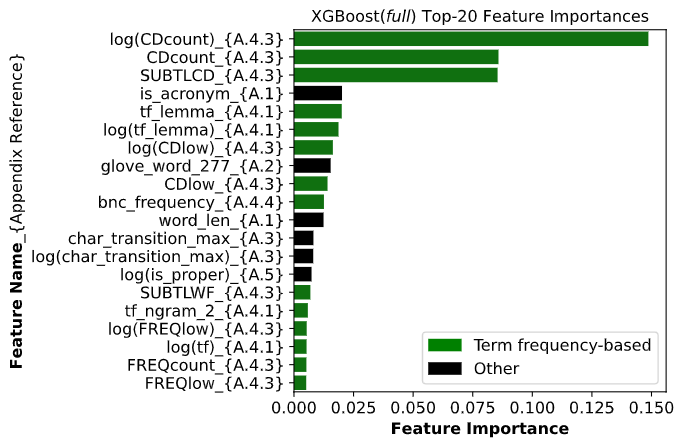
\includegraphics[scale=0.45]{xgboost_feature_importances.png}
  \captionsetup{justification=centering}
  \caption{\label{fig:xgboost_feature_importance} Feature importances for XGBoost(\textit{full}).}
\end{figure}

In total we consider 110 features, in addition to our embedding-based features and $\log$ transformed features. We inspect the estimated feature importance scores produced by the XGBoost(\textit{full}) model to find that term frequency-based features (eg. unigrams, bigrams, trigrams) are of overwhelming importance (see Figure \ref{fig:xgboost_feature_importance}). This inspires concern over whether the MT-DNN model too relies on term frequencies to make \textit{its} predictions, and if not, the linguistic features it may have learned upon fine-tuning. Note that of the remaining features with non-zero importances, the majority seem to be dimensions of one of target word-based semantic features (ie. GloVe or ELMo embeddings).

\subsection{BERT Attention}

\begin{figure}
  \centering
  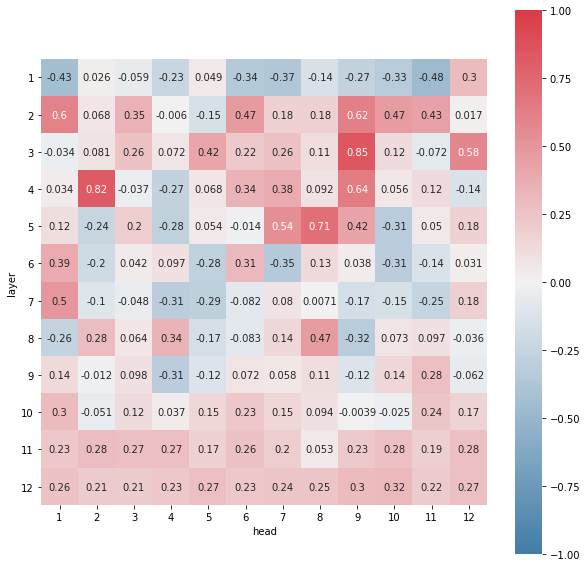
\includegraphics[scale=0.375]{head_correlations_tf.png}
  \captionsetup{justification=centering}
  \caption{\label{fig:head_correlations_tf} Attention head correlation between word frequency and total attention received by word, averaged across 100 random test set samples.}
\end{figure}

\begin{figure}
  \centering
  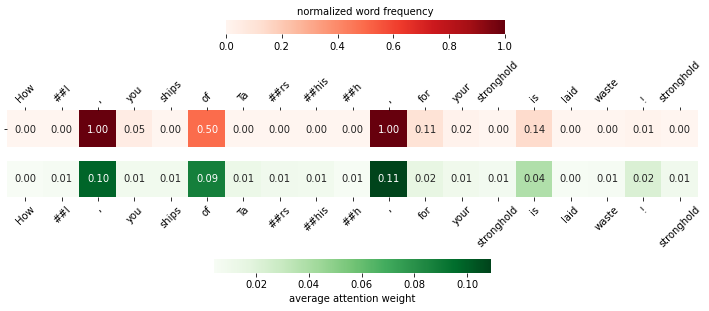
\includegraphics[scale=0.3]{head_3-9_tf_avg.png}
  \captionsetup{justification=centering}
  \caption{\label{fig:head_3-9_tf_avg} Word frequency vs. average head 3-9 attention weight directed to words of a random sample.}
\end{figure}

\begin{figure}
  \centering
  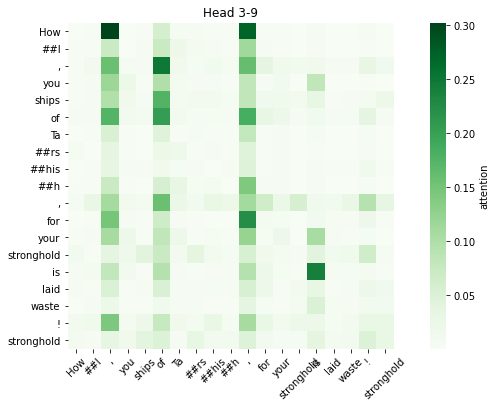
\includegraphics[scale=0.45]{head_3-9.png}
  \captionsetup{justification=centering}
  \caption{\label{fig:head_3-9} Head 3-9 attention map for a random sample.}
\end{figure}

The attention maps of Transformers have in previous works been assessed to demonstrate linguistic phenomena potentially learned by specialized attention heads \citep{1905-09418, 1906-04341} and to measure the relative contribution of each attention head to making task predictions \citep{1905-09418, 1905-10650}. We thereby hope to provide intuition for the MT-DNN model by extracting attention maps from its underlying fine-tuned BERT architecture. For each sample in the single word test set, we extract an attention map from each of the BERT base model's 144 attention heads (ie. 12 heads per 12 layers).

Based on the precedence given to term frequency features by our XGBoost(\textit{full}) model, we hypothesize that for certain attention heads, the degree to which tokens are attended to varies relative to the token's rarity in the lexicon. This follows the findings of \citealp{1905-09418}, who identify heads in which lesser frequent tokens are attended to uniformly by the majority of sentence tokens. 

To test our hypothesis, we estimate for each attention head the Pearson correlation between word frequency and the average attention given to each word in the sentence.\footnote{We compute attention given to a \textit{word} as the sum of attention given to its constituent \textit{byte pair encodings} (BPEs). We use the Google Book Ngram Dataset to extract term frequencies from, though any large corpora would suffice.} As illustrated in Figures \ref{fig:head_correlations_tf} and \ref{fig:head_3-9_tf_avg}, we find multiple attention heads specializing in direct attention towards the most \textit{or} least frequent words (depending on sign of the correlation). Vertical, striated patterns like that in Figure \ref{fig:head_3-9} emerge as a result of attention originating from a spectrum of tokens. Reasoning for the variation across each vertical stripe remains inconclusive, however. The findings are intruiging nonetheless, as they affirm the fundamental relevancy of term frequency to lexical complexity prediction, as our intuition may tell us.

\section{Conclusion \& Future Work}
\begin{itemize}
  \item Any avenues for improvement, including synthetic data generation to improve Pearson correlation on extremely difficult samples, one may also considered extracting sentence embeddings, formed by summing the outputs of the final 4 layers of BERT, alas we leave this for future research.
\end{itemize}

\bibliographystyle{acl_natbib}
\bibliography{anthology,acl2021}

%\appendix

\end{document}
